\section{Actividad 3}

\subsection*{Se tiene la función de densidad de la Fig.~\ref{fig:diagrama_3}}

\begin{figure}[H]
    \centering
    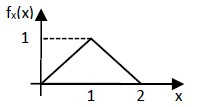
\includegraphics[width=0.35\linewidth]{imagenes/Actividad_3/actividad_3.jpg}
    \caption{Función de densidad triangular.}
    \label{fig:diagrama_3}
\end{figure}

La función de densidad se describe analíticamente como:
\[
f_X(x)=
\begin{cases}
x, & 0 \leq x \leq 1, \\[6pt]
2-x, & 1 < x \leq 2, \\[6pt]
0, & \text{otro caso}.
\end{cases}
\]

%---------------------------------------------------------
\subsection*{a) Calcular analíticamente la media, la varianza y la desviación estándar.}

	La media es:
	\[
		\mu_x = \int_{-\infty}^{\infty} x f_X(x)\, dx
		= \int_{0}^{1} x \cdot x \, dx + \int_{1}^{2} x \cdot (2-x) \, dx
		= \int_{0}^{1} x^2 \, dx + \int_{1}^{2} (2x - x^2)\, dx
	\]
	
	\[
		= \int_{0}^{1} x^2 \, dx + \left( \int_{1}^{2} 2x \, dx - \int_{1}^{2} x^2 \, dx \right)
		= \left. \frac{x^3}{3} \right|_{0}^{1} + \left( \left. x^2 \right|_{1}^{2} - \left. \frac{x^3}{3} \right|_{1}^{2} \right)
	\]
	
	\[
		= \frac{1}{3} + \left[ (4-1) - \left( \frac{8}{3} - \frac{1}{3} \right) \right]
		= \frac{1}{3} + \left( 3 - \frac{7}{3} \right)
		= \frac{1}{3} + \frac{2}{3} = 1
	\]
	
	La varianza es: 
	\[
		\sigma_x^2 = \int_{-\infty}^{\infty} (x - \mu_x)^2 f_X(x)\, dx
		= \int_{0}^{1} (x-1)^2 x \, dx + \int_{1}^{2} (x-1)^2 (2-x)\, dx
	\]
	
	\[
		= \int_{0}^{1} (x^2 - 2x + 1)x \, dx + \int_{1}^{2} (x^2 - 2x + 1)(2-x)\, dx
	\]
	
	\[
		= \int_{0}^{1} (x^3 - 2x^2 + x) \, dx + \int_{1}^{2} (2x^2 - 4x + 2 - x^3 + 2x^2 - x)\, dx
	\]
	
	\[
		= \int_{0}^{1} (x^3 - 2x^2 + x) \, dx + \int_{1}^{2} (-x^3 + 4x^2 - 5x + 2)\, dx
	\]
	
	\[
		= \left[ \frac{x^4}{4} - \frac{2x^3}{3} + \frac{x^2}{2} \right]_{0}^{1}
		+ \left[ -\frac{x^4}{4} + \frac{4x^3}{3} - \frac{5x^2}{2} + 2x \right]_{1}^{2}
	\]
	
	\[
		= \frac{1}{12} + \left( \frac{2}{3} - \frac{7}{12} \right) - \frac{1}{12} + \frac{1}{12}
		= \frac{1}{6}
	\]
	
	Por último, la desviación estandar se calcula como la raíz cuadrada positiva de la varianza $\sigma_x^{2}$, entonces:
	
	\[
		\sigma_x = \sqrt{\sigma_x^2} = \sqrt{\tfrac{1}{6}} \approx 0.4082
	\]
	

%---------------------------------------------------------
\subsection*{b) Calcular y graficar la función de distribución acumulada.}

 La función de distribucion se define como:
 
 \[
 	 F_X(x) = \int_{-\infty}^{0} f_x (t) \, dt 
 \]
 
 Por lo tanto, realizando los cálculos correspondientes se tiene que: 
 

\begin{itemize}
	\item Para $x \leq 0$:
	\[
	F_X(x) = \int_{-\infty}^{0} 0 \, dt = 0
	\]
	
	\item Para $0 \leq x \leq 1$:
	\[
	F_X(x) = \int_{0}^{x} t \, dt 
	= \left. \frac{t^2}{2} \right|_{0}^{x} 
	= \frac{x^2}{2}
	\]
	
	\item Para $1 \leq x \leq 2$:
	\[
	F_X(x) = \int_{0}^{1} t \, dt + \int_{1}^{x} (2-t)\, dt
	= \left. \frac{t^2}{2} \right|_{0}^{1} + \left. \left(2t - \frac{t^2}{2}\right) \right|_{1}^{x}
	\]
	\[
	= \frac{1}{2} + \left(2x - \frac{x^2}{2} - 2 + \frac{1}{2}\right)
	= 2x - \frac{x^2}{2} - 1
	\]
	
	\item Para $x > 2$:
	\[
	F_X(x) = \int_{0}^{1} t \, dt + \int_{1}^{2} (2-t)\, dt 
	= \frac{1}{2} + \left(4 - 2 - \frac{3}{2}\right) 
	= 1
	\]
\end{itemize}
 
 Finalmente se obtiene que la función de distribución acumulada es: 
 
 \[
	 F_X(x) =
		 \begin{cases}
		 	0, & x \leq 0 \\[6pt]
		 	\dfrac{x^2}{2}, & 0 \leq x \leq 1 \\[6pt]
		 	2x - \dfrac{x^2}{2} - 1, & 1 \leq x \leq 2 \\[6pt]
		 	1, & x \geq 2
		 \end{cases}
	 \]

    En la Fig.\ref{fig:4b} se puede observar que la función de distribución acumulada es nula para valores menores o iguales 0 y posee amplitud unitaria 
    para valores mayores o iguales a 2.\par

        \begin{figure}[H]
            \centering
            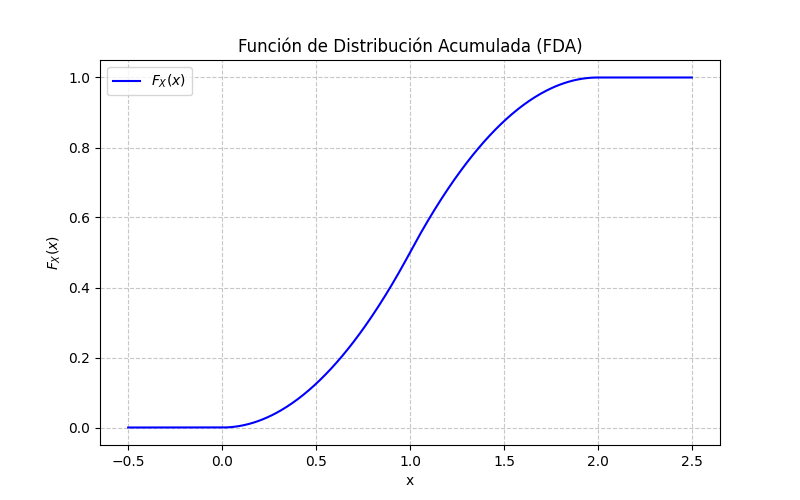
\includegraphics[width=0.7\linewidth]{imagenes/Actividad_3/distribucion_acumulada.png}
            \caption{Función de distribución acumulada \(F_X(x)\).}
            \label{fig:4b}
        \end{figure}

%---------------------------------------------------------
\subsection*{c) Calcular de la probabilidad \( P(0.75 \leq X \leq 1.75) \)}

	Para determinar la probabilidad de que la variable aleatoria \(X\) se encuentre en el intervalo \([0.75, 1.75]\), se utiliza la propiedad fundamental de la función de distribución acumulada (FDA):
	
	\[
		P(a \leq X \leq b) = F_X(b) - F_X(a)
	\]
	
	Aplicando esta propiedad:
	
	\[
		P(0.75 \leq X \leq 1.75) = F_X(1.75) - F_X(0.75)
	\]
	
	Primero, evaluamos la FDA en \(x = 0.75\), correspondiente al intervalo \([0,1]\):
	
	\[
		F_X(0.75) = \frac{0.75^2}{2} = 0.28125
	\]
	
	Luego, evaluamos la FDA en \(x = 1.75\), correspondiente al intervalo \([1,2]\):
	
	\[
		F_X(1.75) = 2(1.75) - \frac{(1.75)^2}{2} - 1 = 0.96875
	\]
	
	Finalmente, reemplazando en la expresión de la probabilidad:
	
	\[
		P(0.75 \leq X \leq 1.75) = 0.96875 - 0.28125 = 0.6875
	\]

	
%---------------------------------------------------------
\subsection*{d) Realizar un código que permita generar vector de 500 muestras aleatorias y graficar el histograma de esas muestras. Luego calcular la media 
	y la varianza.}
	
	
	En la Fig.\ref{fig:4d} se muestra el histograma de 500 muestras aleatorias generado en python. Además, en la Fig.\ref{fig:var_med} se muestran los resultados obtenidos de la media y la varianza, dichos resultados se obtienen de aplicar las funciones mean() para el cálculo de la media y la función var() para el cálculo de la varianza, estas funciones de encuentran en la biblioteca numpy. 
	
	\begin{figure}[H]
		\centering
		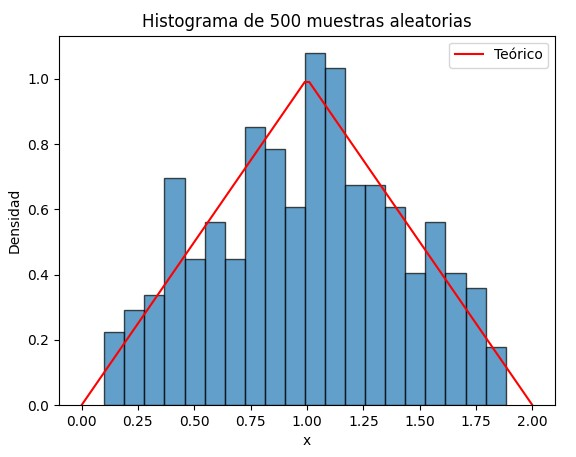
\includegraphics[width=0.6\linewidth]{imagenes/Actividad_3/histograma.jpg}
		\caption{Histograma.}
		\label{fig:4d}
	\end{figure}
	
	
	\begin{figure}[H]
		\centering
		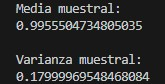
\includegraphics[width=0.3\linewidth]{imagenes/Actividad_3/var_med.jpg}
		\caption{Varianza y media.}
		\label{fig:var_med}
	\end{figure}

